% Beamer presentation
\documentclass[11pt,aspectratio=43,ignorenonframetext,t]{beamer}

% Presentation settings
\mode<presentation>{
  \usetheme[framenumber,titleframestart=1]{UoM_alex}
  \usefonttheme{professionalfonts} % using non standard fonts for beamer
  \usefonttheme{serif}
  \usepackage{fontspec}
  \setmainfont[Ligatures=TeX]{Arial}
}

% Handout settings
\mode<article>{
  \usepackage{fullpage}
  \usepackage{fontspec}
  \setmainfont[Ligatures=TeX]{Arial}
  \setlength{\parskip}{1.5\baselineskip} % correct beamer line spacings
  \setlength{\parindent}{0cm}
  \usepackage{enumitem}
  \setlist[itemize]{topsep=0pt}
}

 % Packages
\usepackage{graphicx}
\graphicspath{{./images/png}} % generic graphics path; overridden if necessary
\usepackage{amsmath}
\allowdisplaybreaks[1] % allow eqnarrays to break across pages
\usepackage{amssymb} 
\usepackage[HTML]{xcolor}
\definecolor{uomlinkblue}{HTML}{0071BC}
\usepackage{hyperref}
\hypersetup{
  colorlinks=true,
  linkcolor=uomlinkblue,
  filecolor=uomlinkblue,      
  urlcolor=uomlinkblue,
  pdflang={en-GB},
}
\usepackage[document]{ragged2e} % left aligned text for accessibility
\usepackage{tikz}
\usetikzlibrary{positioning, arrows, arrows.meta}
\usepackage{unicode-math} % unicode maths for accessibility
\usepackage{pdfcomment}   % for alt text for accessibility
\usepackage{rotating}     % allow portrait figures and tables
\usepackage{subfigure}    % allow matrices of figures
\usepackage{float}        % allows H option on floats to force here placement
\usepackage{multirow}     % allows merging of rows in tables
\usepackage{tabularx}     % allows fixed width tables
\usepackage{ctable}       % modifies \hline for use in table
\usepackage{bm}           % allow bold fonts in equations
\usepackage{pgf}          % allow graphics manipulation
\usepackage{etoolbox}
  
% Custom commands
\newcolumntype{Z}{>{\centering\arraybackslash}X}  % tabularx centered columns 

\makeatletter
  \DeclareRobustCommand{\em}
  {
    \@nomath\em
    \if b
      \expandafter\@car\f@series\@nil \normalfont
    \else
      \bfseries
    \fi
  }
\makeatother

\makeatletter
  \preto{\@verbatim}{\topsep=0pt \partopsep=0pt}
\makeatother

\def\checkmark{
  \tikz\fill[scale=0.4](0,.35) -- (.25,0) -- (1,.7) -- (.25,.15) -- cycle;
}

% Counters
\newcounter{example_number} % keep track of the example questions

% Frontmatter
\newcommand{\cmclecture}[1]{
  \title{Combinatorial Mesh Calculus (CMC): Lecture #1}
}
\author{
  Lectured by:
  \href{https://scholar.google.com/citations?user=x4R-snQAAAAJ&hl=en}
  {Dr. Kiprian Berbatov}$^1$\\
  \smallskip
  Lecture Notes Compiled by:
  \href{https://scholar.google.com/citations?user=CoIpITkAAAAJ&hl=en}
  {Muhammad Azeem}$^1$\\
  \smallskip
  Under the supervision of:
  \href{https://scholar.google.co.uk/citations?user=3nWJe5wAAAAJ&hl=en}
  {Prof. Andrey P. Jivkov}$^1$\\
  \smallskip
  {\tiny $^1$Department of Mechanical and Aerospace Engineering,
    The University of Manchester, Oxford Road, Manchester M13 9PL, UK}
}

% Special frames
\newcommand{\cmctitleframe}{
  \titlepage
  \begin{tikzpicture}[remember picture,overlay]
    \node[anchor=south east] at (current page.south east) {
      \href{https://youtube.com/@kipi.berbatov}{
        \includegraphics[width=1.5cm]{youtube-icon.png}
      }
    };
  \end{tikzpicture}
}
\newcommand{\cmcendframe}{
  \begin{figure}
    \centering
    \includegraphics[width=0.85\linewidth]{Thanks.png}
  \end{figure}
}

\cmclecture{16}
\date{07 November 2025}

\usepackage{tikz}
\usetikzlibrary{calc}
\usepackage{booktabs}

\begin{document}

%========================= TITLE =========================
\begin{frame}
  \cmctitleframe
\end{frame}

\begin{frame}{Setup: Continuous–Discrete Analogy for Transport Phenomena}
\begin{block}{Geometric Context}
Let \((M,g)\) be an oriented, compact, smooth Riemannian manifold and
\((K,\mu)\) be an oriented, finite Riemannian quasi–cubical mesh partition of \(M\).
Both have equal topological dimension \(D=\dim K=\dim M\).
\end{block}

\begin{block}{Summary}
This setup establishes a parallel between the smooth differential structure of \(M\)
and its discrete combinatorial representation on \(K\), where forms correspond to cochains, and exterior derivatives correspond to coboundary operators.
\end{block}
\end{frame}

\begin{frame}{Setup: Continuous - Discrete}

\begin{block}{Spaces and Operations}
\vspace{-0.3cm}
\begin{center}
\resizebox{\textwidth}{!}{%
\begin{tabular}{c|c|c}
\toprule
\textbf{Category} & \textbf{Exterior Calculus (EC)} & \textbf{Combinatorial Mesh Calculus (CMC)}\\
\midrule
Chains & -- & $C_{\bullet}K$\\
Cochains / Forms & $\Omega^{\bullet}M$ & $C^{\bullet}K$\\
Product & $\wedge: \Omega^pM\times\Omega^qM\to\Omega^{p+q}M$ & $\smile: C^pK\times C^qK\to C^{p+q}K$\\
Differential & $d_p:\Omega^pM\to\Omega^{p+1}M$ & $\delta_p:C^pK\to C^{p+1}K$\\
Integration & $\displaystyle \int_M:\Omega^DM\to\mathbb{R}$ & $\displaystyle \int_{[K]}:C^DK\to\mathbb{R},\;
\sigma[K]=\sum_{c\in K_D}\sigma(c)$\\
\bottomrule
\end{tabular}
}
\end{center}
\end{block}

\end{frame}


\begin{frame}{Metric–Dependent Operators in EC and CMC}
\vspace{-0.3cm}
\begin{block}{Operators on Forms and Cochains}
\vspace{-0.3cm}
\begin{center}
\resizebox{\textwidth}{!}{%
\vspace{-0.3cm}
\begin{tabular}{c|c|c}
\toprule
\textbf{Operator} & \textbf{Exterior Calculus (EC)} & \textbf{Combinatorial Mesh Calculus (CMC)}\\
\midrule
Pointwise Metric & $g_p^*: \Omega^pM\times\Omega^pM\to \mathcal{F}(M)$ & --\\
Inner Product & $\langle\cdot,\cdot\rangle_p:\Omega^pM\times\Omega^pM\to\mathbb{R}$ & $\langle\cdot,\cdot\rangle_p^K:C^pK\times C^pK\to\mathbb{R}$\\
Hodge Star & $\star_p:\Omega^pM\to\Omega^{D-p}M$ & $\star_p^K:C^pK\to C^{D-p}K$\\
Adjoint Differential & $d_p^*:\Omega^pM\to\Omega^{p-1}M$ & $\delta_p^*:C^pK\to C^{p-1}K$\\
\bottomrule
\end{tabular}
}
\end{center}
\end{block}

\vspace{-0.5cm}
\begin{block}{Fundamental Equalities}
\vspace{-0.7cm}
\begin{align*}
&\langle \star_p\omega, \eta\rangle = \int_M \omega\wedge\eta,
&&\langle \star_p^K\sigma, \rho\rangle^K = (\sigma\smile\rho)[K],\\[3pt]
&\langle d_p^*\omega, \eta\rangle_{p-1} = \langle\omega, d_{p-1}\eta\rangle_p,
&&\langle \delta_p^*\sigma, \rho\rangle_{p-1}^K = \langle\sigma, \delta_{p-1}\rho\rangle_p^K,\\[3pt]
&d^*_{D-p}\circ\star_p = (-1)^{p+1}\star_{p+1}\circ d_p,
&&\delta^*_{D-p}\circ\star_p^K = (-1)^{p+1}\star_{p+1}^K\circ\delta_p.
\end{align*}
\vspace{-0.3cm}
\end{block}
\end{frame}


\begin{frame}{Algebraic Identities and Relations}
\vspace{-0.3cm}
\begin{block}{Product Properties}
\vspace{-0.7cm}
\begin{align*}
\omega\wedge\eta = & (-1)^{pq}\eta\wedge\omega,\\
\sigma\smile\rho = & (-1)^{pq}\rho\smile\sigma,\\
d(\omega\wedge\eta) = &d\omega\wedge\eta + (-1)^p\omega\wedge d\eta,\\
\delta(\sigma\smile\rho) = &\delta\sigma\smile\rho + (-1)^p\sigma\smile\delta\rho.
\end{align*}
\end{block}
\vspace{-0.3cm}
\begin{block}{Integration and Stokes–Type Relation}
\vspace{-0.3cm}
\begin{align*}
&\int_M d\omega = \int_{\mathrm{tr}_{\partial M}}\omega,
&&(\delta\sigma)[K] = \sigma(\partial[K]),\\
&[K] = \sum_{c\in K_D} c_\bullet,
&&\partial[K] \text{ contains only boundary } (D-1)\text{–cells.}
\end{align*}
\end{block}

\end{frame}

\begin{frame}{Differences}

\begin{block}{Remarks}
\begin{enumerate}
    \item The wedge product is associative, while the cup product is only graded–commutative but not associative.\\
    \item \(\star_p\) is invertible with \(\star_p\circ\star_{D-p}=(-1)^{p(D-p)}\mathrm{id}\),
whereas \(\star_p^K\) is not invertible in general since \(|K_p|\neq|K_{D-p}|\).
\end{enumerate}
\end{block}
\end{frame}





\begin{frame}{Special Cases of the Hodge Star}
\vspace{-0.3cm}
\begin{block}{Conditions of Invertibility}
In special cases, discrete Hodge stars are invertible:
\vspace{-0.3cm}
\begin{align*}
&\star_0^K\mathbb{1}
= \sum_{c\in K_D}\mu(c)c^\bullet
= \mathrm{vol},\\
&\star_D^K(\mathrm{vol}) = \mathbb{1}.
\end{align*}
On a regular cubical grid, cochains can be formed by summing all cells aligned along the same direction,
yielding sign–consistent duals.
\end{block}

\vspace{-0.3cm}
\begin{block}{Orientation Relation on Regular Grids}
\vspace{-0.3cm}
\begin{align*}
&\star_p^K \sigma^{p,(i_1,\dots,i_p)}
=\pm \sigma^{D-p,(i_1,\dots,i_{D-p})},
\\
&(i_1,\dots,i_p)\cup(i_1,\dots,i_{D-p})=\{1,\dots,D\}.
\end{align*}
\end{block}
\end{frame}


\begin{frame}{Example: Hodge Stars}
\vspace{-0.3cm}
\begin{block}{Mesh Description}
A $2\times2$ square mesh with vertices $N_0,\dots,N_8$,
edges $E_0,\dots,E_{11}$, and faces $F_0,\dots,F_3$.
All faces are counterclockwise oriented.

Edge measures:
\vspace{-0.7cm}
\begin{align*}
\mu(E_0)=\cdots=\mu(E_5)=x,\\
\mu(E_6)=\cdots=\mu(E_{11})=y,\\
\mu(F_0)=\cdots=\mu(F_3)=xy.
\end{align*}

\vspace{-1.1cm}
\begin{align*}
\star_0^K\sigma^0
&=\sum_{c\in K_2}\mu(c)c^\bullet
=\sum_{i=0}^{3}xy\,F_i^\bullet,\\
\star_1^K\sigma^{1,(1)}
&=\frac{y}{2}\sum_{j=6}^{11}E_j^\bullet,\qquad
\star_1^K\sigma^{1,(2)}=\frac{x}{2}\sum_{j=0}^{5}E_j^\bullet,\\
\star_2^K\sigma^{2,(1,2)}
&=\frac{1}{4xy}\sum_{v=0}^{8}N_v^\bullet.
\end{align*}
\end{block}
\end{frame}

\begin{frame}{Example: Hodge Stars}
    \begin{block}{Summary}
The discrete Hodge star exchanges primal and dual components
with scaling factors derived from local measures \(\mu(c)\).
\end{block}
\vspace{-0.2cm}
\begin{block}{Primal Mesh and Orientation}
\begin{center}
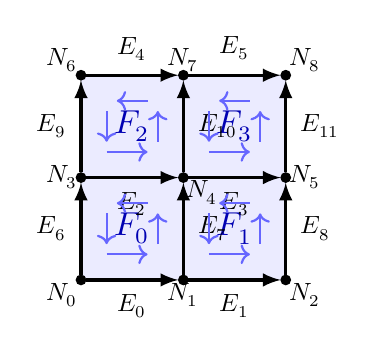
\begin{tikzpicture}[scale=1.3, every node/.style={font=\small}]
% --- Draw grid background ---
\foreach \i in {0,1,2}{
  \draw[gray!40,thin] (\i,0)--(\i,2);
  \draw[gray!40,thin] (0,\i)--(2,\i);
}

% --- Highlight faces ---
\fill[blue!8] (0,1) rectangle (1,2);
\fill[blue!8] (1,1) rectangle (2,2);
\fill[blue!8] (0,0) rectangle (1,1);
\fill[blue!8] (1,0) rectangle (2,1);

% --- Vertices ---
\foreach \i/\x/\y/\pos in {0/0/0/below left, 1/1/0/below, 2/2/0/below right,
                            3/0/1/left, 4/1/1/below right, 5/2/1/right,
                            6/0/2/above left, 7/1/2/above, 8/2/2/above right}{
  \fill (\x,\y) circle (1.5pt);
  \node[\pos,inner sep=1pt] at (\x,\y) {$N_{\i}$};
}

% --- Face labels ---
\node[blue!70!black,font=\large] at (0.5,0.5) {$F_0$};
\node[blue!70!black,font=\large] at (1.5,0.5) {$F_1$};
\node[blue!70!black,font=\large] at (0.5,1.5) {$F_2$};
\node[blue!70!black,font=\large] at (1.5,1.5) {$F_3$};

% --- Horizontal edges (bottom row) ---
\draw[very thick,->,>=latex] (0.05,0)--(0.95,0);
\node[below] at (0.5,-0.05) {$E_0$};

\draw[very thick,->,>=latex] (1.05,0)--(1.95,0);
\node[below] at (1.5,-0.05) {$E_1$};

% --- Horizontal edges (middle row) ---
\draw[very thick,->,>=latex] (0.05,1)--(0.95,1);
\node[below] at (0.5,0.95) {$E_2$};

\draw[very thick,->,>=latex] (1.05,1)--(1.95,1);
\node[below] at (1.5,0.95) {$E_3$};

% --- Horizontal edges (top row) ---
\draw[very thick,->,>=latex] (0.05,2)--(0.95,2);
\node[above] at (0.5,2.05) {$E_4$};

\draw[very thick,->,>=latex] (1.05,2)--(1.95,2);
\node[above] at (1.5,2.05) {$E_5$};

% --- Vertical edges (left column) ---
\draw[very thick,->,>=latex] (0,0.05)--(0,0.95);
\node[left] at (-0.05,0.5) {$E_6$};

\draw[very thick,->,>=latex] (0,1.05)--(0,1.95);
\node[left] at (-0.05,1.5) {$E_9$};

% --- Vertical edges (middle column) ---
\draw[very thick,->,>=latex] (1,0.05)--(1,0.95);
\node[right] at (1.05,0.5) {$E_7$};

\draw[very thick,->,>=latex] (1,1.05)--(1,1.95);
\node[right] at (1.05,1.5) {$E_{10}$};

% --- Vertical edges (right column) ---
\draw[very thick,->,>=latex] (2,0.05)--(2,0.95);
\node[right] at (2.05,0.5) {$E_8$};

\draw[very thick,->,>=latex] (2,1.05)--(2,1.95);
\node[right] at (2.05,1.5) {$E_{11}$};

% --- Orientation arrows (counterclockwise on each face) ---
\foreach \cx/\cy in {0.5/0.5, 1.5/0.5, 0.5/1.5, 1.5/1.5}{
  \draw[->,blue!60,thick] (\cx-0.25,\cy-0.25)--(\cx+0.15,\cy-0.25);
  \draw[->,blue!60,thick] (\cx+0.25,\cy-0.15)--(\cx+0.25,\cy+0.15);
  \draw[->,blue!60,thick] (\cx+0.15,\cy+0.25)--(\cx-0.15,\cy+0.25);
  \draw[->,blue!60,thick] (\cx-0.25,\cy+0.15)--(\cx-0.25,\cy-0.15);
}
\end{tikzpicture}
\end{center}
\end{block}

\end{frame}

\begin{frame}{Transport Phenomena: EC Formulation}
\vspace{-0.2cm}
\begin{block}{Geometric and Setup}
Let \(I=[t_0,\infty)\) be the time interval and \(M\) be a compact, oriented,
Riemannian \(D\)-dimensional manifold representing the spatial domain.
The boundary is decomposed as
\vspace{-0.5cm}
\begin{align*}
\partial M = \Gamma_D \cup \Gamma_N,
\qquad \Gamma_D \cap \Gamma_N = \emptyset.
\end{align*}
\end{block}
\vspace{-0.4cm}
\begin{block}{Known Variables and Parameters}
\vspace{-0.7cm}
\begin{align*}
&V: I \to \Omega^{D-1}M\to\ \text{Volumetric flow rate (advective velocity)},\\
&f: I \to \Omega^{D}M\to\ \text{Internal production rate},\\
&g_D: I \to \Omega^{0}\Gamma_D\to\ \text{Dirichlet boundary (prescribed potential)},\\
&g_N: I \to \Omega^{D-1}\Gamma_N\to\ \text{Neumann boundary (prescribed flow rate)},\\
&u_0 \in \Omega^{0}M\to\ \text{Initial potential},
\end{align*}
\end{block}
\end{frame}

\begin{frame}{Transport Phenomena: EC Formulation}
\vspace{-0.2cm}
\begin{block}{Known Variables and Parameters}
\vspace{-0.7cm}
\begin{align*}
&\kappa: C^\infty(I,\Omega^{D-1}M)\!\to\! C^\infty(I,\Omega^{D-1}M)\to\ \text{Conductivity},\\
&\tilde{\kappa}: C^\infty(I,\Omega^{1}M)\!\to\! C^\infty(I,\Omega^{1}M)\to\ \text{Dual conductivity},\\
&\pi: C^\infty(I,\Omega^{D}M)\!\to\! C^\infty(I,\Omega^{D}M)\to\ \text{Capacity},\\
&\tilde{\pi}: C^\infty(I,\Omega^{0}M)\!\to\! C^\infty(I,\Omega^{0}M)\to\ \text{Dual apacity}.
\end{align*}
\end{block}

\begin{block}{Physical Meaning}
\(\kappa,\tilde{\kappa}\) are conductivities (or transport parameter),
\(\pi,\tilde{\pi}\) are capacities. They relate fluxes and potentials through the metric–dependent Hodge star.
\end{block}
\end{frame}


\begin{frame}{Variables in the EC Formulation}
\vspace{-0.2cm}

\begin{block}{Unknown Variables (Field Quantities)}
\vspace{-0.7cm}
\begin{align*}
u: I &\to \Omega^{0}M, &
&\text{Potential (scalar field)},\\
Q: I &\to \Omega^{D}M, &
&\text{Amount (total stored content)},\\
q: I &\to \Omega^{D-1}M, &
&\text{Flux (diffusive + advective flow)}.
\end{align*}
\vspace{-0.2cm}
\begin{align*}
&\text{Relations:}\quad
Q = \pi\,\star_0 u,\qquad
q = -\,\star_1\,\tilde{\kappa}\, d_0 u + \star_D(Q)\wedge V.
\end{align*}
\end{block}

\vspace{-0.2cm}
\begin{block}{Summary}
The unknowns \((u, q, Q)\) evolve in time,
driven by the given transport parameters \((\kappa,\tilde{\kappa},\pi,\tilde{\pi})\)
and boundary/initial conditions \((g_D, u_0)\).
\end{block}
\end{frame}


\begin{frame}{Governing Equations in Exterior Calculus}
\begin{block}{Continuity and Conservation Laws}
\vspace{-0.7cm}
\begin{align*}
\frac{\partial Q}{\partial t} &= f - d_{D-1}q,\\
\frac{\partial Q}{\partial t} &= \pi \star_0 \frac{\partial u}{\partial t},\\
\star_D\frac{\partial Q}{\partial t} &= \tilde{\pi}\frac{\partial u}{\partial t}.
\end{align*}
The first equation expresses local conservation,
while the second and third express material capacity through potential variation.
\end{block}
\end{frame}

\begin{frame}{Governing Equations in Exterior Calculus}
\begin{block}{Constitutive and Advective Relations}
\vspace{-0.7cm}
\begin{align*}
q_D &= \kappa\, d_D \star_0 u
\;=\;
-\,\star_1\,\tilde{\kappa}\, d_0 u,\\
q_A &= \star_D(Q)\wedge V.
\end{align*}
Here \(q_D\) is the diffusive flux and \(q_A\) the advective contribution.
\end{block}

\begin{block}{Boundary and Initial Conditions}
\vspace{-0.3cm}
\begin{align*}
\operatorname{tr}_{\Gamma_{N,D-1}}(q) &= g_N,\\
\operatorname{tr}_{\Gamma_{D,0}}(u) &= g_D,\\
u(t_0)&=u_0.
\end{align*}
\end{block}
\end{frame}


\begin{frame}{CMC Analogue}
\vspace{-0.2cm}
\begin{block}{Discrete Setting}
Let \((K,\mu)\) be an oriented, finite, Riemannian quasi–cubical mesh
partitioning \(M\) with \(\dim K = D\).
Each smooth quantity has a discrete counterpart on \(K\).
\end{block}

\begin{block}{Discrete Variables and Parameters}
\vspace{-0.8cm}
\begin{align*}
&V^K: I \to C^{D-1}K,\\
&f^K: I \to C^{D}K,\\
&g_D^K: I \to C^{0}\Gamma_D,\\
&u_0^K \in C^{0}K,\\
&\kappa^K: C^\infty(I,C^{D-1}K)\to C^\infty(I,C^{D-1}K),\\
&\tilde{\kappa}^K: C^\infty(I,C^{1}K)\to C^\infty(I,C^{1}K),\end{align*}
\end{block}
\end{frame}

\begin{frame}{CMC Analogue}
\vspace{-0.2cm}

\begin{block}{Discrete Variables and Parameters}
\vspace{-0.3cm}
\begin{align*}
&\pi^K: C^\infty(I,C^{D}K)\to C^\infty(I,C^{D}K),\\
&\tilde{\pi}^K: C^\infty(I,C^{0}K)\to C^\infty(I,C^{0}K).
\end{align*}
All these operators encode discrete transport parameters derived from metric information.
\end{block}

\vspace{-0.3cm}

\begin{block}{Unknown Variables (Field Quantities)}
\vspace{-0.7cm}
\begin{align*}
u^K: I &\to C^{0}K, &
&\text{Potential},\\
Q^K: I &\to C^{D}K, &
&\text{Amount (total stored content)},\\
q^K: I &\to C^{D-1}K, &
&\text{Flux (diffusive + advective flow)}.
\end{align*}
\end{block}
\end{frame}

\begin{frame}{Governing Equations in the CMC}
\vspace{-0.3cm}
\begin{block}{Discrete Continuity and Constitutive Laws}
\vspace{-0.3cm}
\begin{align*}
\frac{\partial Q^K}{\partial t} &= f^K - \delta_{D-1} q^K,\\
\frac{\partial Q^K}{\partial t} &= \pi^K \star_0^K \frac{\partial u^K}{\partial t},\\
\star_D^K \frac{\partial Q^K}{\partial t} &= \tilde{\pi}^K \frac{\partial u^K}{\partial t},\\
q_D^K &= \kappa^K \, \delta_D \star_0^K u^K
= -\,\star_1^K \tilde{\kappa}^K \delta_0 u^K,\\
q_A^K &= \star_D^K(Q^K)\smile V^K.
\end{align*}
The operators \(\delta_p\) are discrete coboundaries,
and \(\smile\) replaces the wedge product.
\end{block}
\end{frame}

\begin{frame}{Boundary Conditions}
    \begin{block}{Boundary and Initial Conditions}
\vspace{-0.3cm}
\begin{align*}
\operatorname{tr}_{\Gamma_{N,D-1}}(q^K) &= g_N^K,\\
\operatorname{tr}_{\Gamma_{D,0}}(u^K) &= g_D^K,\\
u^K(t_0) &= u_0^K.
\end{align*}
\end{block}
\end{frame}


\begin{frame}{Remarks on Metric Non–Invertibility}
\vspace{-0.3cm}
\begin{block}{Hodge–Star Non–Invertibility}
Unlike the smooth case, the discrete Hodge stars are not necessarily invertible:
\vspace{-0.3cm}
\begin{align*}
\star_p^K: C^pK \to C^{D-p}K
\quad \text{is non–invertible since } |K_p| \neq |K_{D-p}|.
\end{align*}
Consequently, the discrete transport tensors
\(\kappa^K, \tilde{\kappa}^K, \pi^K, \tilde{\pi}^K\)
cannot in general be inverted exactly.
\end{block}

\begin{block}{Summary}
The CMC formulation mirrors the EC equations via algebraic operators on cochains, replacing differential and integral structures with incidence–based and combinatorial ones. Metric effects and transport coefficients are captured through the discrete Hodge star and measure weighting.
\end{block}
\end{frame}


\begin{frame}{Primal Weak Formulation in EC}
\vspace{-0.1cm}
\begin{block}{Test Function Space}
Choose a test function
\vspace{-0.3cm}
\begin{align*}
w \in \operatorname{Ker} \operatorname{tr}_{\Gamma_D,0}
= \{\omega \in \Omega^0 M \mid \operatorname{tr}_{\Gamma_D,0}\omega = 0\}
= \{\omega \in \mathcal{F}M \mid \omega|_{\Gamma_D}=0\}.
\end{align*}
\textbf{Multiplying the Conservation Law:} Multiply \(w\) with the conservation equation and integrate over \(M\):
\vspace{-0.3cm}
\begin{align*}
\int_M w \wedge \frac{\partial Q}{\partial t}
&= -\!\int_M w \wedge d_{D-1}q + \!\int_M (w \wedge f),\\
&= -\!\int_{\partial M} \!\operatorname{tr}_{\partial M,D-1}(w \wedge q)
+ \!\int_M (d_0w \wedge q) + \!\int_M (w \wedge f),\\
&= -\!\int_{\Gamma_N} (\operatorname{tr}_{\Gamma_N,0} w \wedge g_N)
- \langle d_0 w,\tilde{\kappa} d_0 u\rangle_{M,1}\\&
+ \!\int_M (d_0w \wedge \tilde{\pi} u \wedge V)
+ \!\int_M (w \wedge f).
\end{align*}
\vspace{-0.5cm}
\end{block}
\end{frame}


\begin{frame}{Weak Formulation}
\begin{block}{Amount–Potential Coupling}
Multiplying \(w\) with the constitutive relation for the amount gives:
\vspace{-0.3cm}
\begin{align*}
\int_M w \wedge \frac{\partial Q}{\partial t}
= \int_M w \wedge (\star_0 \tilde{\pi} \frac{\partial u}{\partial t})
= \langle w, \tilde{\pi} \frac{\partial u}{\partial t} \rangle_{M,0}.
\end{align*}
Equating both sides yields the primal weak formulation of the EC transport model.
\end{block}

\begin{block}{Interpretation}
The weak formulation balances local conservation and material accumulation,
respecting Dirichlet and Neumann boundary conditions through test functions.
\end{block}
\end{frame}


\begin{frame}{Operator Formulation of EC Weak Model}
\vspace{-0.2cm}
\begin{block}{Operator Definitions}
\vspace{-0.3cm}
\begin{align*}
A_D(w,u) &:= \langle d_0w, \tilde{\kappa} d_0u\rangle_{M,1},\\
A_A(w,u) &:= \int_M (d_0w \wedge (\tilde{\pi}u \wedge V)),\\
B(w,u) &:= \langle w, \tilde{\pi}u\rangle_{M,0},\\
G(w) &:= \int_{\Gamma_N} (\operatorname{tr}_{\Gamma_N,0} w \wedge g_N),\\
F(w) &:= \int_M (w \wedge f).
\end{align*}
\end{block}
\end{frame}

\begin{frame}{Operator Formulation of EC Weak Model}
\vspace{-0.2cm}

\begin{block}{Weak Problem}
Find \(u[Y]\in C^\infty(I,\Omega^0 M)\) such that for all
\(w[Y]\in \operatorname{Ker}\operatorname{tr}_{\Gamma_D,0}\),
\vspace{-0.3cm}
\begin{align*}
B(w,\tfrac{\partial u}{\partial t})
+ A_D(w,u)
- A_A(w,u)
= F(w) - G(w),
\end{align*}
with boundary and initial conditions
\begin{align*}
\operatorname{tr}_{\Gamma_D,0}(u) = g_D, \qquad u(t_0)=u_0.
\end{align*}
\end{block}
\end{frame}

\begin{frame}{Post–Processing: Flow Rate in EC}
\begin{block}{Computed Quantity}
Once \(u\) is obtained, the flow rate is reconstructed as:
\vspace{-0.3cm}
\begin{align*}
q(t,x) =
\begin{cases}
(-\star_1 \tilde{\kappa} d_0 u + \tilde{\pi} u \wedge V)(t,x),
& x \notin \Gamma_N,\, t\in I,\\
g_N(t,x), & x\in \Gamma_N,\, t\in I.
\end{cases}
\end{align*}
\end{block}

\begin{block}{Remark}
Steady–state formulations arise when \(\frac{\partial}{\partial t}\) is ignored,
and all quantities become time–independent.
\end{block}
\end{frame}


\begin{frame}{Primal Weak Formulation in CMC}
\begin{block}{Discrete Operators}
By direct translation of EC operators:
\vspace{-0.3cm}
\begin{align*}
A_D^K(w^K,u^K)&:=\langle \delta_0 w^K, \tilde{\kappa}^K \delta_0 u^K\rangle_{K,1},\\
A_A^K(w^K,u^K)&:=\sum_{c\in K_D}(\delta_0w^K\smile(\tilde{\pi}^K u^K\smile V^K))[c],\\
B^K(w^K,u^K)&:=\langle w^K,\tilde{\pi}^K u^K\rangle_{K,0},\\
G^K(w^K)&:=\sum_{b\in \Gamma_N}(w^K\smile g_N^K)[b],\\
F^K(w^K)&:=\sum_{c\in K_D}(w^K\smile f^K)[c].
\end{align*}
\end{block}
\end{frame}

\begin{frame}{Primal Weak Formulation in CMC}
\begin{block}{Discrete Weak Problem}
Find \(u^K[Y^K]\) such that
\vspace{-0.3cm}
\begin{align*}
B^K(w^K,\tfrac{\partial u^K}{\partial t})
+ A_D^K(w^K,u^K)
- A_A^K(w^K,u^K)
= F^K(w^K)-G^K(w^K),
\end{align*}
with
\begin{align*}
\operatorname{tr}_{\Gamma_D,0}(u^K)=g_D^K,\qquad u^K(t_0)=u_0^K.
\end{align*}
\end{block}
\end{frame}

\begin{frame}{Remarks on CMC Approximation and Post–Processing}
\vspace{-0.3cm}
\begin{block}{Approximation Note}
The equality
\(\langle \star\sigma, \star\rho \rangle = \langle \sigma, \rho \rangle\)
is only approximate in CMC since the discrete Hodge stars are non–invertible.
This approximation is accepted in simulations.
\end{block}

\begin{block}{Post–Processing}
After computing \(u^K\):
\vspace{-0.3cm}
\begin{align*}
q^K = \star_1^K \tilde{\kappa}^K \delta_0 u^K,
\end{align*}
valid in the interior (\(x\notin\Gamma_N\)).
This step introduces numerical errors because it depends
on non–invertible discrete Hodge maps.
\end{block}
\end{frame}


\begin{frame}{Mixed Weak Formulation in EC}

\begin{block}{Test Function and Constitutive Relation}
Choose
\vspace{-0.3cm}
\begin{align*}
r \in \operatorname{Ker}(\operatorname{tr}_{\Gamma_N,D-1})
= \{s \in \Omega^{D-1}M \mid \operatorname{tr}_{\Gamma_N,D-1}s=0\}.
\end{align*}
Rewrite the constitutive law:
\vspace{-0.3cm}
\begin{align*}
\kappa^{-1} q_D = d_D^*\star_0 u = -\star_1 d_0 u.
\end{align*}
Taking the inner product yields
\vspace{-0.3cm}
\begin{align*}
\langle r, \kappa^{-1}q_D\rangle_{M,D-1}
&= -\int_{\Gamma_D} (g_D \wedge \operatorname{tr}_{\Gamma_D,D-1}r)
+\langle d_{D-1}r,\tilde{u}\rangle_{M,D-1}\\&
+\langle r, \kappa^{-1}(\star_D \tilde{\pi}\tilde{u}\wedge V)\rangle_{M,D-1}.
\end{align*}
\end{block}
\end{frame}


\begin{frame}{Mixed Weak Formulation (Operator Representation)}
\vspace{-0.3cm}
\begin{block}{Operators}
\vspace{-0.3cm}
\begin{align*}
A(r,s)&:=\langle r, \kappa^{-1}s\rangle_{M,D-1},\\
B_D(\tilde{w},r)&:=\langle d_{D-1}r,\tilde{w}\rangle_{M,D},\\
B_A(\tilde{w},r)&:=\langle r,\kappa^{-1}(\star_D\tilde{\pi}\tilde{w}\wedge V)\rangle_{M,D-1},\\
C(\tilde{w},\tilde{u})&:=\langle \tilde{\pi}\tilde{u},\tilde{w}\rangle_{M,D},\\
G(r)&:=\int_{\Gamma_D}(\operatorname{tr}_{\Gamma_D,D-1}r \wedge g_D),\\
F(\tilde{w})&:=\langle f,\tilde{w}\rangle_{M,D}.
\end{align*}
\end{block}
\end{frame}

\begin{frame}{Mixed Weak Formulation (Operator Representation)}

\begin{block}{Weak Problem}
Find \(q,\tilde{u}\) such that:
\vspace{-0.3cm}
\begin{align*}
A(r,q)-B_D^T(r,\tilde{u})-B_A^T(r,\tilde{u})&=-G(r),\\
-B_D(\tilde{w},q)-C(\tilde{w},\tfrac{\partial \tilde{u}}{\partial t})&=-F(\tilde{w}),
\end{align*}
with
\begin{align*}
\operatorname{tr}_{\Gamma_N,D-1}q = g_N,\quad
\tilde{u}(t_0)=\star_0 u_0,\quad
q(t_0)=\kappa d_D^*\star_0 u_0 + \pi u_0\wedge V.
\end{align*}
\end{block}
\end{frame}

\begin{frame}{Mixed Weak Formulation in CMC}
\begin{block}{Discrete System}
By literal translation of EC operators:
\vspace{-0.3cm}
\begin{align*}
A^K(r^K,s^K)&:=\langle r^K,(\kappa^K)^{-1}s^K\rangle_{K,D-1},\\
B_D^K(\tilde{w}^K,r^K)&:=\langle \delta_{D-1}r^K,\tilde{w}^K\rangle_{K,D},\\
B_A^K(\tilde{w}^K,r^K)&:=\langle r^K,(\kappa^K)^{-1}(\star_D^K\tilde{\pi}^K\tilde{w}^K\smile V^K)\rangle_{K,D-1},\\
C^K(\tilde{w}^K,\tilde{u}^K)&:=\langle \tilde{\pi}^K\tilde{u}^K,\tilde{w}^K\rangle_{K,D}.
\end{align*}
The boundary and source terms \(G^K, F^K\) are discretised analogously.
\end{block}

\end{frame}


\begin{frame}{Mixed Weak Formulation in CMC}

\begin{block}{Discrete Weak Problem}
Find \(q^K, \tilde{u}^K\) such that:
\vspace{-0.3cm}
\begin{align*}
A^K(r^K,q^K)-B_D^{K,T}(r^K,\tilde{u}^K)-B_A^{K,T}(r^K,\tilde{u}^K)
&=-G^K(r^K),\\
-B_D^K(\tilde{w}^K,q^K)-C^K(\tilde{w}^K,\tfrac{\partial \tilde{u}^K}{\partial t})
&=-F^K(\tilde{w}^K),
\end{align*}
with
\begin{align*}
\operatorname{tr}_{\Gamma_N,D-1}q^K=g_N^K,\quad
\tilde{u}^K(t_0)=\star_0^K u_0^K,\quad
q^K(t_0)=\text{flow\_rate}^K(u_0^K).
\end{align*}
\end{block}
\end{frame}

\begin{frame}{Post–Processing and Remarks on the Mixed Formulation}
\vspace{-0.3cm}
\begin{block}{Post–Processing in the Interior}
Once \(q^K, \tilde{u}^K\) are found, the interior potential can be reconstructed as:
\vspace{-0.3cm}
\begin{align*}
u^K = \star_D^K \tilde{u}^K.
\end{align*}
\end{block}
\vspace{-0.3cm}
\begin{block}{Remarks}
\begin{itemize}
\item The CMC system is a literal discrete translation of the EC formulation.
\item Post–processing may accumulate errors due to non–invertibility of
\(\star_p^K\).
\item The relation
\(\langle \star\sigma, \star\rho\rangle = \langle\sigma,\rho\rangle\)
is not exact in CMC but is used as an approximation in simulations.
\end{itemize}
\end{block}
\end{frame}


\begin{frame}{Summary}
\vspace{-0.2cm}

\begin{block}{1. Mathematical Setting}
We model transport phenomena on an oriented, compact Riemannian manifold \((M,g)\)
and its discrete counterpart — an oriented Riemannian quasi–cubical mesh \((K,\mu)\),
with \(\dim M = \dim K = D\).
The smooth and discrete theories correspond via:
\[
\Omega^\bullet M \leftrightarrow C^\bullet K,\quad
d_p \leftrightarrow \delta_p,\quad
\wedge \leftrightarrow \smile,\quad
\star_p \leftrightarrow \star_p^K.
\]
\end{block}
\end{frame}


\begin{frame}{Summary}
\vspace{-0.2cm}
\begin{block}{2. Metric and Algebraic Structure}
Both settings admit inner products, Hodge stars, and adjoint operators:
\begin{align*}
\langle \star_p\omega,\eta\rangle &= \int_M \omega\wedge\eta, &
\langle \star_p^K\sigma,\rho\rangle^K &= (\sigma\smile\rho)[K],\\
d_p^* &= (-1)^{p+1}\star_{p+1} d_p \star_{D-p}, &
\delta_p^* &= (-1)^{p+1}\star_{p+1}^K \delta_p \star_{D-p}^K.
\end{align*}
Unlike the smooth case, discrete Hodge stars are non–invertible,
so \(\langle \star\sigma,\star\rho\rangle = \langle \sigma,\rho\rangle\) holds only approximately.
\end{block}

\end{frame}


\begin{frame}{Summary}
\begin{block}{3. Governing Equations}
\textbf{Continuity:}
\(\displaystyle \frac{\partial Q}{\partial t} = f - d_{D-1}q.\)
\quad
\textbf{Constitutive:}
\(q = -\star_1\tilde{\kappa}d_0u + \star_D(Q)\wedge V.\)
\quad
\textbf{Capacity:}
\(Q = \pi\star_0u = \star_D^{-1}\tilde{\pi}u.\)

Boundary and initial data:
\begin{align*}
\operatorname{tr}_{\Gamma_N,D-1}q &= g_N, &
\operatorname{tr}_{\Gamma_D,0}u &= g_D, &
u(t_0) &= u_0.
\end{align*}
\end{block}
\end{frame}



\begin{frame}{Summary}
\vspace{-0.2cm}
\begin{block}{4. Primal Weak Formulation (EC)}
Using test functions \(w\in\operatorname{Ker} \operatorname{tr}_{\Gamma_D,0}\):
\begin{align*}
B(w,\tfrac{\partial u}{\partial t})
+ A_D(w,u) - A_A(w,u)
= F(w) - G(w),
\end{align*}
where
\begin{align*}
A_D(w,u)&=\langle d_0w,\tilde{\kappa}d_0u\rangle_{M,1}, &
A_A(w,u)&=\int_M d_0w\wedge(\tilde{\pi}u\wedge V),\\
B(w,u)&=\langle w,\tilde{\pi}u\rangle_{M,0}, &
G(w)&=\int_{\Gamma_N}\!(\operatorname{tr}_{\Gamma_N,0}w\wedge g_N),\\
F(w)&=\int_M(w\wedge f).
\end{align*}
The post–processed flow is
\(q = -\star_1\tilde{\kappa}d_0u + \tilde{\pi}u\wedge V.\)
\end{block}
\end{frame}


\begin{frame}{Summary}
\begin{block}{5. Primal Weak Formulation (CMC)}
A literal discrete translation replaces
\((d,\wedge,\star)\) by \((\delta,\smile,\star^K)\).
Post–processing yields
\(q^K = \star_1^K\tilde{\kappa}^K\delta_0u^K\),
which introduces small errors since \(\star_p^K\) is not invertible.
\end{block}
\begin{block}{6. Mixed EC Formulation}
Using test functions
\(r\in\operatorname{Ker}(\operatorname{tr}_{\Gamma_N,D-1})\) and \(\tilde{w}\in\Omega^D M\):
\begin{align*}
A(r,q) - B_D^T(r,\tilde{u}) - B_A^T(r,\tilde{u}) &= -G(r),\\
-B_D(\tilde{w},q) - C(\tilde{w},\tfrac{\partial\tilde{u}}{\partial t}) &= -F(\tilde{w}),
\end{align*}
with
\(\tilde{u} = \star_0u\),
\(\operatorname{tr}_{\Gamma_N,D-1}q=g_N\),
and
\(q(t_0)=\kappa d_D^*\star_0u_0+\pi u_0\wedge V.\)
\end{block}

\end{frame}


\begin{frame}{Summary}
\vspace{-0.2cm}

\begin{block}{7. Mixed CMC Formulation}
Discrete system obtained by direct translation:
\begin{align*}
A^K(r^K,q^K) - B_D^{K,T}(r^K,\tilde{u}^K) - B_A^{K,T}(r^K,\tilde{u}^K)
&= -G^K(r^K),\\
-B_D^K(\tilde{w}^K,q^K) - C^K(\tilde{w}^K,\tfrac{\partial\tilde{u}^K}{\partial t})
&= -F^K(\tilde{w}^K).
\end{align*}
The interior potential is reconstructed by
\(u^K = \star_D^K \tilde{u}^K.\)
\end{block}
\end{frame}



\begin{frame}{Conceptual Overview}
\vspace{-0.2cm}
\begin{block}{8. Key Insights}
\begin{itemize}
\item Exterior Calculus (EC) provides a coordinate–free continuous formulation of transport.
\item Combinatorial Mesh Calculus (CMC) discretises EC exactly at the algebraic level.
\item Smooth differential operators \((d, \star, \wedge)\) correspond to discrete ones
\((\delta, \star^K, \smile)\).
\item Weak formulations (primal and mixed) preserve local conservation and boundary flux balance.
\item Post–processing reconstructs flux or potential but introduces minor errors due to
non–invertible \(\star_p^K\).
\end{itemize}
\end{block}
\end{frame}


\begin{frame}{Summary}
\begin{block}{9. Summary Remark}
Discrete formulations in CMC are not approximations of EC \emph{by projection},
but algebraic translations preserving structure and topology —
offering a unified geometric language for numerical transport models.
\end{block}
\end{frame}


\begin{frame}{Thanks}
  \cmcendframe
\end{frame}

\end{document}
